\documentclass[leqno]{beamer}
\usetheme{Madrid}
\usecolortheme{seahorse}

\usepackage[linesnumbered,algoruled,boxed,lined]{algorithm2e}
\usepackage{amsfonts,amsmath,amssymb}
\usepackage{bbm}
\usepackage{booktabs}
\usepackage{caption}
\usepackage{color}
\usepackage{graphicx}
\graphicspath{{./}{../image/}} % graphic path
\usepackage{hyperref}
\hypersetup{colorlinks,citecolor=blue,linkcolor=[RGB]{50,50,172}}
\usepackage{multicol}
\usepackage{multirow}
\usepackage[authoryear]{natbib}
\usepackage{setspace}
\usepackage{soul}
\usepackage{textpos}
\usepackage{tikz}

%% notations; only define those you use frequently
\newcommand{\EE}{{\mathbb{E}}}
\newcommand{\PP}{{\mathbb{P}}}
\newcommand{\QQ}{{\mathbb{Q}}}
\newcommand{\Fb}{\mathbf{F}}
\newcommand{\Ib}{\mathbf{I}}
\newcommand{\hb}{\mathbf{h}}
\newcommand{\xb}{\mathbf{x}}
\newcommand{\one}{\mathbbm{1}}
\newcommand{\Ocal}{\mathcal{O}}

% consistent with R manual
\newcommand\pkg[1]{\texttt{#1}}
\let\proglang=\textsf \let\code=\texttt

\setbeamercovered{transparent}
\setbeamertemplate{caption}[numbered]
\setbeamertemplate{enumerate item}[default]
\setbeamertemplate{itemize item}[circle]
\setbeamertemplate{section in toc}[default]
\setbeamertemplate{subsection in toc}[default]

\AtBeginSection[]{
\begin{frame}<beamer>{Overview}
\tableofcontents[currentsection]
\end{frame}}


\title[\textcolor{black}{UNet-HCRF\_EEG}]{\large
UNet-HCRF Integration for Sequence Labeling on EEG Data}

\author[\scalebox{.85}{Xiaohang Ma, Shiying Xiao, Xiaohui Yin}]
{Xiaohang Ma$^1$, Shiying Xiao$^2$, Xiaohui Yin$^2$}

\institute[\scalebox{.85}{UConn}]
{$^1$Department of Mathematics, University of Connecticut \\
$^2$Department of Statistics, University of Connecticut}

\date[December 9, 2024]{
{\small Storrs, CT} \\
{\small December 9, 2024}}

\begin{document}

\begin{frame}[plain]
\titlepage
\end{frame}


\begin{frame}
\frametitle{Overview}
\tableofcontents
\end{frame}


\section[Introduction]{Introduction}


\begin{frame}{Introduction}
\begin{itemize}
\setlength{\itemsep}{1.5em}
\item Sequence labeling tasks are crucial for healthcare, where accurate and
timely data classification can significantly impact patient outcomes.
\item Deep learning has recently emerged as a powerful tool for sequence
labeling.
\item Conditional random fields (CRFs) have been employed for modeling label
dependencies, demonstrating promising results.
\end{itemize}
\end{frame}


\section[Methods]{Methods}


\begin{frame}{CNN-HCRF Model Structure}
\begin{itemize}
\item An UNet CNN was designed to generate a feature map, and a global
potential for the label.
\item A hidden conditional random field (HCRF) layer processes the pixel-wise
label information from the feature map, assigning a latent label $h_i$ to each
pixel.
\item The latent label $h_i$ contributes to the global feature through the
following potetial:
\begin{equation*}
\varphi(y, h_{j}; \delta) = \sum_{a \in Y} \sum_{b \in H} \delta_{a, b}
\cdot \one(y = a) \cdot \one(h_j = b),
\end{equation*}
where $\delta_{a,b}$ denotes the likelihood of class label $y = a$
containing a joint with hidden state $h_j = b$, learned during training.
\end{itemize}
\end{frame}


\begin{frame}{CNN-HCRF Model Structure (cont.)}
\begin{small}
\begin{itemize}
\item Unary potential $\phi(h_j, x_j; \omega)$: Measures the likelihood of the
local feature $x_j$ is assigned as the hidden part state $h_j$, whose parameter
$\omega$ is learned by end-to-end CNN-UNet structure.
\item Binary potential $\psi(h_i, h_j, x_i, x_j; \eta)$: Balances the hidden
label compatibility of the neighboring pixels $p$ on the feature image 
$\Fb(\Ib)$:
\begin{align*}
\psi(h_i, h_j, x_i, x_j; \eta) &= \mu(h_i, h_j) \Bigg[
\omega_1 \exp \left(
-\frac{\left\lvert p_i - p_j \right\rvert^2}{2\eta_\alpha^2}
-\frac{\left\lvert \Fb_i(\Ib) - \Fb_j(\Ib) \right\rvert^2}{2\eta_\beta^2}
\right) \\
&+ \omega_2 \exp \left(
- \frac{\left\lvert p_i - p_j \right\rvert^2}{2 \eta_\gamma^2}
\right)
\Bigg],
\end{align*}
where the parameters $\eta_\alpha$, $\eta_\beta$ and $\eta_\gamma$ control the
influence of the corresponding feature spaces.
\item Global potential $\vartheta(y, \xb; \varpi)$: Measures the compatibility
of class label $y$ and the global feature vector $x_0$ of the whole action,
whose parameter $\varpi$ will be learned during training process.
\end{itemize}
\end{small}
\end{frame}


\begin{frame}{CNN-HCRF Model Structure (cont..)}
Let $y$ represent the corresponding label of the input image $\xb$.
The jointly probability distribution of the HCRF model is:
\begin{align*}
\Phi(y, \hb, \xb; \theta) &= \underbrace{
\sum_{j \in \nu} \phi(h_j, x_j; \omega) +
\sum_{i \neq j} \psi(h_i, h_j, x_i, x_j; \eta)}_{
% \propto \log\PP( \hb \vert \xb; \theta)
\textrm{Measures log-likelihood $\log\PP(\hb \vert \xb; \theta)$}} \\
& + \underbrace{
\sum_{j \in \nu} \varphi(y, h_j, x_j; \delta) + \vartheta(y, \xb; \varpi)}_{
% \propto \log\PP(y | \hb, \xb; \theta)
\textrm{Measures log-likelihood $\log\PP(y \vert \hb, \xb; \theta)$}}
\end{align*}
\end{frame}


%\begin{frame}{Model Structure}
%\begin{small}
%\begin{itemize}
%\item An Unet CNN was designed to generated a feature map, and a global
%potential for the label.
%\item A hidden CRF layer will address the pixel wise label information of the
%feature map, then assign a latent label $h_i$ at each pixel.
%\item The latent label $h_i$ will contribute the global feature through the
%following potetial.
%\begin{equation*}
%\varphi(y, h_{j}; \delta) = \sum_{a \in Y} \sum_{b \in H} \delta_{a, b}
%\cdot \one(y = a) \cdot \one(h_j = b)
%\end{equation*}
%\item The jointly probability distribution of the model
%\begin{equation*}
%\begin{split}
%\Phi(y, \hb, \xb; \theta) &= \underbrace{
%\sum_{j \in \nu} \phi(h_j, x_j; \omega)
%+ \sum_{i \neq j} \psi(h_i, h_j, x_i, x_j; \eta)}_{
%% \propto \log\PP(\hb \vert \xb; \theta)
%\textrm{Measures log-likelihood $\log\PP(\hb \vert \xb; \theta)$}} \\
%&+ \underbrace{
%\sum_{j \in \nu} \varphi(y, h_j, x_j; \delta) + \vartheta(y, \xb; \varpi)}_{
%% \propto \log\PP(y | \hb,  \xb; \theta)
%\textrm{Measures log-likelihood $\log\PP(y \vert \hb, \xb; \theta)$}}
%\end{split}
%\end{equation*}
%\end{itemize}
%\end{small}
%\end{frame}


\begin{frame}{Model Inference}
\begin{small}
\begin{itemize}
\item The inference for the latent variable follows a standard mean-field
Variational Inference scheme.
\begin{equation*}
\QQ(h_i) \propto \exp\{\EE_{\QQ(\hb_{-i})}
\log\PP(y, h_i, \hb_{-i} \vert \xb; \theta)\}.
\end{equation*}
\item The resulting ELBO will be used as predicted log-likelihood of each image:
\begin{equation*}
\begin{split}
& \textrm{ELBO}(\QQ) = \EE_{\QQ(\hb)} \log\PP(y, \hb \vert \xb; \theta)
- \EE_{\QQ(\hb)} \log q(\hb) \\
&\quad = \sum_{i=1}^N \EE_{q_i(h_i)}
\left[ \phi(h_j, x_j; \omega) + \varphi(y, h_j, x_j; \delta) \right] \\
&\quad + \sum_{i=1}^N \sum_{j=1}^N \sum_{l,l^\prime} \one_{\{i \neq j\}} 
\QQ(h_i = l) \QQ(h_j = l^\prime) \mu(l, l^\prime) \\
&\quad \left[ \omega_1 \exp \left(
- \frac{\left\lvert p_i - p_j \right\rvert^2}{2\eta_\alpha^2}
- \frac{\left\lvert \Fb_i(\Ib) - \Fb_j(\Ib) \right\rvert^2}{2\eta_\beta^2}
\right) + \omega_2 \exp \left(
- \frac{\left\lvert p_i - p_j \right\rvert^2}{2\eta_\gamma^2}
\right) \right] \\
&\quad - \sum_{i=1}^N \EE_{q_i} \log q_i(h_i) + \vartheta(y, \xb; 
\varpi).
\end{split}
\end{equation*}
\end{itemize}
\end{small}
\end{frame}


\section[Data Preprocessing]{Data Preprocessing}


\begin{frame}{Data Preparation}
\begin{itemize}
\item Extract the 10 min long Kaggle Spectrogram centered at the middle time
where the experts rating (Global EEGs)
\item Transform the 50s long EEG waveforms into Spectrograms
\end{itemize}
\end{frame}


\begin{frame}{EEG signal denosing using Wavelet transform}
\begin{footnotesize}
\begin{align*}
& \text{LL Spec} = \frac{1}{4} \left[
spec(Fp1-F7) + spec(F7-T3) + spec(T3-T5) + spec(T5-O1) \right], \\
& \text{LP Spec} = \frac{1}{4} \left[
spec(Fp1-F3) + spec(F3-C3) + spec(C3-P3) + spec(P3-O1) \right], \\
& \text{RP Spec} = \frac{1}{4} \left[
spec(Fp2-F4) + spec(F4-C4) + spec(C4-P4) + spec(P4-O2) \right], \\
& \text{RR Spec} = \frac{1}{4} \left[
spec(Fp2-F8) + spec(F8-T4) + spec(T4-T6) + spec(T6-O2) \right]
\end{align*}
\end{footnotesize}
\begin{figure}[tbp]
\centering
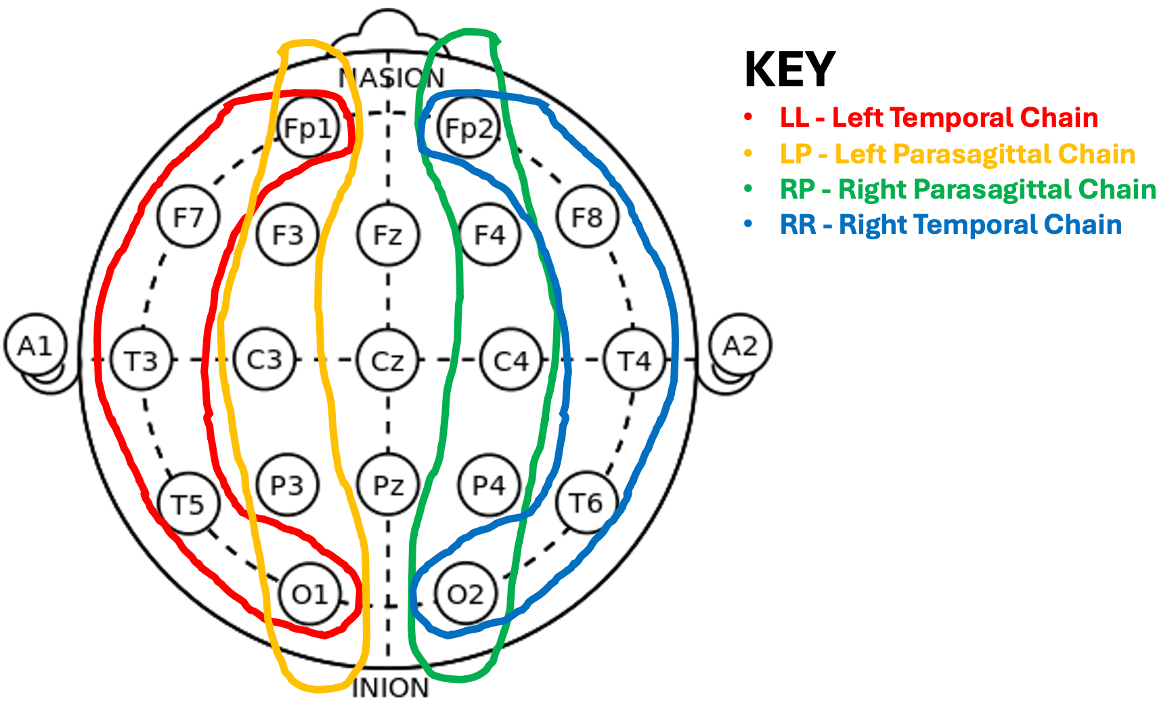
\includegraphics[width=.55\textwidth]{inion}
\end{figure}
\end{frame}


\begin{frame}{EEG Signal Denosing using Wavelet Transform}
\begin{enumerate}
\item Calculates the mean absolute deviation of a signal $d$:
\begin{equation*}
\mathrm{maddest}(d, axis) = \frac{1}{N} \sum_{i=1}^N
\left\vert d_i - \frac{1}{N} \sum_{j=1}^N d_j \right\vert,
\end{equation*}
where $d_i$ is the value of the signal at index $i$, and
$N$ is the length of $d$.
\item Denoises a signal using wavelet decomposition:
\begin{enumerate}
\item Perform wavelet decomposition
\item Calculate the noise standard deviation using the last level of
coefficients
\item Compute the universal threshold
\item Apply a hard thresholding operation to the coefficients
\item Reconstruct the signal using the inverse wavelet transform
\end{enumerate}
\end{enumerate}
\end{frame}


\begin{frame}{Create Spectrograms from the Middle 50 Seconds}
\begin{figure}[tbp]
\centering
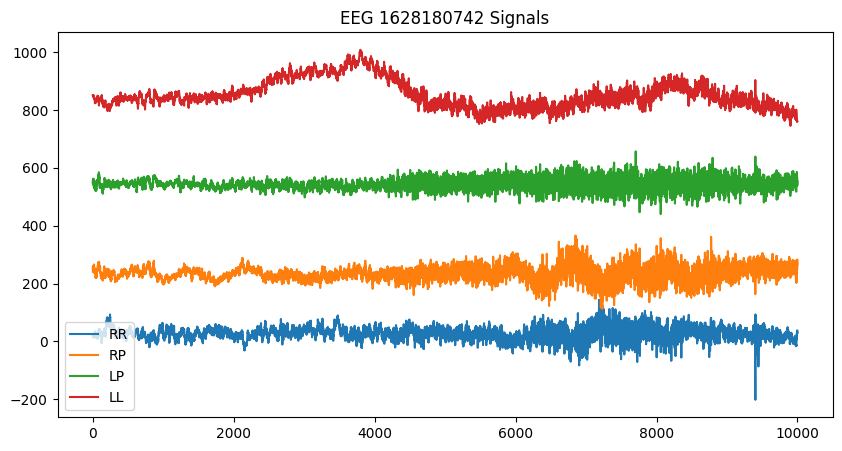
\includegraphics[width=.4\textwidth]{EEG_Signal}
\end{figure}
\begin{figure}[tbp]
\centering
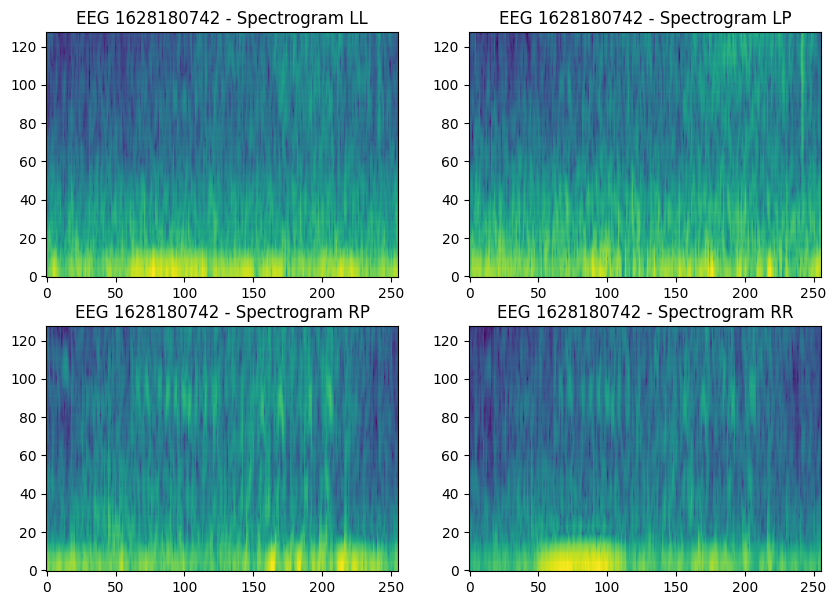
\includegraphics[width=.5\textwidth]{EEG_Spectrogram}
\end{figure}
\end{frame}















%\begin{frame}[allowframebreaks]
%\frametitle{References}
%\bibliographystyle{plain}
%\bibliography{bib}
%\end{frame}

\end{document}
%%% Local Variables:
%%% mode: latex
%%% TeX-master: t
%%% End:
